%*******************************************************************************************%
%	   CONTRIBUIÇÕES À MODELAGEM DINAMICA E AO CONTROLE DE MANIPULADORES PARALELOS          %
% 																					   		%
% June 2015															 						%
% Author: Renato Maia Matarazzo Orsino														%
% bash modularmodelling.sh					 												%
% 																							%
%*******************************************************************************************%


\documentclass[25pt,landscape]{beamer}
	\mode<presentation> {
	  \usetheme{Warsaw}
	  \setbeamercovered{transparent}
	  \useoutertheme{shadow}
	  \useoutertheme{infolines}
	  \useinnertheme{rounded}
	  \setbeamertemplate{theorems}[numbered]
	  \setbeamertemplate{bibliography item}[text]
	  \usecolortheme{default}
	}


% - INPUT - %
\usepackage[T1]{fontenc}
\usepackage[latin1]{inputenc}


% - MATH - %
\usepackage{amsmath,amsfonts,amssymb}
\usepackage{amsthm}
\usepackage{accents}


% - GENERAL - %
\usepackage{cmbright}
\usepackage{natbib}
\usepackage{color}
% \usepackage[pdftex,dvipsnames]{color}
% \usepackage{geometry}
\usepackage{array,hhline,supertabular,tabularx}
\usepackage{hyperref}
% \usepackage[colorlinks,citecolor=black,urlcolor=black,linkcolor=black]{hyperref}
\usepackage{graphicx}
% \usepackage[pdftex]{graphicx}
\usepackage{enumitem}
\usepackage{float}
\usepackage{titlesec}
\usepackage{pp4link}
\usepackage{mpmulti}
\usepackage{multimedia}
\usepackage[display]{texpower}
\usepackage{multicol}
\usepackage[overlay,absolute]{textpos}
\setlength{\TPHorizModule}{1cm}
\setlength{\TPVertModule}{1cm}
\usepackage{multicol}

% - SPECIAL - %
\usepackage{EXTRAS/special-char}
\usepackage{EXTRAS/special-conf}




%---------------------------------------------------------------------------------------%
%										BEAMER											%
%---------------------------------------------------------------------------------------%

\begin{document}


\begin{frame}
    \titlepage
\end{frame}



%--- INTRODU\c{c}\~aO -------------------------------------------------------------------------%


%\begin{frame}{Test frame}
%    \begin{textblock}{12}(0.4,1.5)
%            \begin{exampleblock}{Answered Questions}
%            \end{exampleblock}
%            \begin{block}{Defini\c{c}\~ao}
%                A \alert{set} consists of elements.
%            \end{block}
%    \end{textblock}
%\end{frame}



\begin{frame}{Motiva\c{c}\~ao}
    \framesubtitle{Mecanismos paralelos}
    \pause
    \begin{block}{Caracter\'isticas Promissoras}
    	\pause
        \begin{itemize} 
            \item[--] Grande capacidade de carga \\[8pt]
            \item[--] Alta rigidez estrutural \\[8pt]
            \item[--] Alta precis\~ao de posicionamento \\[8pt]
            \item[--] Baixa in\'ercia \\[8pt]
            \item[--] Altas velocidades e acelera\c{c}\~oes \\[8pt]
        \end{itemize}
    \end{block}
    \pause
    \begin{block}{Inconveni\^entes}
    	\pause
        \begin{itemize}
        	\item[--] Grande n\'umero de componentes mec\^anicos \\[8pt]
            \item[--] Pequena \'area de trabalho \\[8pt]
            \item[--] Din\^amica complexa e n\~ao linear \\[8pt]
        \end{itemize}
    \end{block}
\end{frame}

\begin{frame}{Motiva\c{c}\~ao}
    \framesubtitle{Mecanismos paralelos}
    \begin{block}{Aplica\c{c}\~oes}
        \begin{itemize}
            \item[--] Pick-and-place
        \end{itemize}
    \end{block}
    \begin{figure}[!h]
        \centering
        \includegraphics[scale=0.35]{ABB-Flexpicker-Robot.png}
    \end{figure}  
\end{frame}

\begin{frame}{Motiva\c{c}\~ao}
    \framesubtitle{Mecanismos paralelos}
    \begin{block}{Aplica\c{c}\~oes}
        \begin{itemize}
            \item[--] Simuladores
        \end{itemize}
    \end{block}
    \begin{figure}[!h]
        \centering
        \includegraphics[scale=0.30]{hexapods.jpg}
    \end{figure}  
\end{frame}

\begin{frame}{Motiva\c{c}\~ao}
    \framesubtitle{Mecanismos paralelos}
    \begin{block}{Aplica\c{c}\~oes}
        \begin{itemize}
            \item[--] Usinagem
        \end{itemize}
    \end{block}
    \begin{figure}[!h]
        \centering
        \includegraphics[scale=0.60]{image44.png}
    \end{figure}  
\end{frame}

%Grupo de pesquisa

\begin{frame}{Motiva\c{c}\~ao}
	\framesubtitle{Grupo de pesquisa}
	\pause
	\begin{block}{Rob\^os}
		Giovanna
    \end{block}
    \begin{figure}[!h]
        \centering
        \includegraphics[scale=0.33]{Giovanna.png}
    \end{figure}
\end{frame}

\begin{frame}{Motiva\c{c}\~ao}
	\framesubtitle{Grupo de pesquisa}
	\begin{block}{Rob\^os}
		Dora
    \end{block}
    \begin{figure}[!h]
        \centering
        \includegraphics[scale=0.33]{Dora.png}
    \end{figure}
\end{frame}

\begin{frame}{Motiva\c{c}\~ao}
	\framesubtitle{Grupo de pesquisa}
	\begin{block}{Rob\^os}
		Laila
    \end{block}
    \begin{figure}[!h]
        \centering
        \includegraphics[scale=0.33]{Laila.jpg}
    \end{figure}
\end{frame}

\begin{frame}{Motiva\c{c}\~ao}
	\framesubtitle{Grupo de pesquisa}
	\begin{block}{Rob\^os}
		Clara
    \end{block}
    \begin{figure}[!h]
        \centering
        \includegraphics[scale=0.2]{Clara2.jpg}
    \end{figure}
\end{frame}

\begin{frame}{Motiva\c{c}\~ao}
	\framesubtitle{Grupo de pesquisa}
	\begin{block}{Clara}
		\begin{itemize}
			\item[$\bullet$] 2015
			\begin{itemize}
				\item[--] B. Ohashi: Síntese dimensional \\[4pt]
				\item[--] V. Bartholomeu: Projeto e contru\c{c}\~ao da estrutura mec\^anica \\[4pt]
			\end{itemize}
			\item[$\bullet$] 2016
			\begin{itemize}
				\item[--] V. Bartholomeu e J. de Oliveira-Fuess: Modelagem e simula\c{c}\~oes cinem\'atica e din\^amica \\[4pt]
			\end{itemize}
			\item[$\bullet$] 2017
			\begin{itemize}
				\item[--] A. Coutinho, V. Bartholomeu e J. de Oliveira-Fuess: Constru\c{c}\~ao do prot\'otipo \\[4pt]
			\end{itemize}
			\item[$\bullet$] 2019
			\begin{itemize}
				\item[--] A. Coutinho: Implementa\c{c}\~ao de t\'ecnicas de controle e ensaios experimentais \\[4pt]
			\end{itemize}
		\end{itemize}
	\end{block}
\end{frame}

\begin{frame}{Motiva\c{c}\~ao}
    \framesubtitle{Metodologia modular de modelagem}
    \pause
    \begin{figure}[!h]
        \centering
        \includegraphics[scale=0.14]{3RRR-1.jpg} \\
        (Orsino 2015)
    \end{figure}  
\end{frame}

\begin{frame}{Motiva\c{c}\~ao}
    \framesubtitle{Controle}
    \pause
    \begin{block}{Controle descentralizado}
    	\pause
        Projeto de controlador de posi\c{c}\~ao para os atuadores, considerando torques do mecanismo como dist\'urbio    
    \end{block}
    \pause
    \begin{exampleblock}{Vantagens}
        \begin{itemize}
            \item[--] Modelagem simples
            %\item[--] \'E poss\'ivel utilizar controle linear
            %\item[--] Projeto de controle relativamente simples
            \item[--] Lei de controle pouco custosa
        \end{itemize}
    \end{exampleblock}
    \pause
    \begin{exampleblock}{Desvantagens}
        \begin{itemize}
            \item[--] Necessita de redutores com altas rela\c{c}\~oes de transmiss\~ao
            \item[--] Desempenho muito limitado
        \end{itemize}
    \end{exampleblock}
\end{frame}

\begin{frame}{Motiva\c{c}\~ao}
    \framesubtitle{Controle}
    \begin{block}{Controle centralizado}
    	\pause
        Projeto de controlador de posi\c{c}\~ao considerando a depend\^encia entre as vari\'aveis controladas (baseado no modelo din\^amico)
    \end{block}
    \pause
    \begin{exampleblock}{Vantagens}
        \begin{itemize}
            \item[--] Maior desempenho: \'e poss\'ivel realizar trajet\'orias em maiores velocidades
            \item[--] Permite utilizar {\em direct drive}
        \end{itemize}
    \end{exampleblock}
    \pause
    \begin{exampleblock}{Desvantagens}
        \begin{itemize}
            \item[--] Modelo din\^amico de dif\'icil obten\c{c}\~ao
            %\item[--] Projeto de controle de maior complexidade
            \item[--] Lei de controle de alto custo computacional
        \end{itemize}
    \end{exampleblock}
\end{frame}

\begin{frame}{Motiva\c{c}\~ao}
    \framesubtitle{Controle}
    \begin{block}{Proposta}
        Tornar poss\'ivel o projeto e implementa\c{c}\~ao de controladores:
        \begin{itemize}
            \item[--]<alert@3> De alto desempenho
            \item[--]<alert@3> Adequados ao controle de trajet\'oria de mecanismos paralelos
            \item[--]<alert@4> Que possam sintetizar leis de controle com menor custo computacional
            \item[--]<alert@4> Alta robustez
        \end{itemize}
    \end{block}
    \pause
    \begin{exampleblock}{Como?}
        \begin{itemize}
            \item[--]<3-> Desenvolvimento e implementa\c{c}\~ao de algoritmo gen\'erico de modelagem e controle de mecanismos paralelos
            \item[--]<4-> Utiliza\c{c}\~ao de t\'ecnicas de controle robusto
        \end{itemize}
    \end{exampleblock}
\end{frame}

\begin{frame}{Motiva\c{c}\~ao}
    \framesubtitle{Controle}
    \begin{table}[H]
        \begin{center}
            \begin{tabular}{|c|c|c|c|c|c|} 
                \hline
                \rule[-2mm]{0mm}{6mm}
                T\'ecnica & Desempenho & Custo & Implement. & Modelagem \\
                \hline
                \rule[-2mm]{0mm}{6mm}
                PID & {\color{red} Baixo} & {\color{blue} Baixo} & {\color{blue} Simples} &  {\color{blue} Simples}    \\
                \rule[-1mm]{0mm}{5mm}
                CTC$^1$ & {\color{orange} M\'edio} & {\color{teal} M\'edio} & {\color{orange} Mediana} & {\color{orange} Mediana}  \\
                \rule[-1mm]{0mm}{5mm}
                Adaptativo$^1$ & {\color{teal} M\'edio/Alto} & {\color{orange} M\'edio/Alto} & {\color{red} Complexa} & {\color{red} Complexa}     \\
                \rule[-1mm]{0mm}{5mm}
                CTC$^2$ & {\color{blue} Alto} & {\color{red} Alto} & {\color{red} Complexa} &  {\color{red} Complexa}  \\
                \rule[-1mm]{0mm}{5mm}
                CMD$^2$ & {\color{blue} Alto} & {\color{teal} M\'edio} & {\color{red} Complexa} & {\color{red} Complexa} \\
                \hline
            \end{tabular}
            %\label{crono}
        \end{center}
    \end{table}
    $$ $$
    1: Modelo simplificado \\
    2: Modelo completo \\
\end{frame}

\begin{frame}{Motiva\c{c}\~ao}
    \framesubtitle{Controle}
    \begin{figure}[!h]
        \centering
        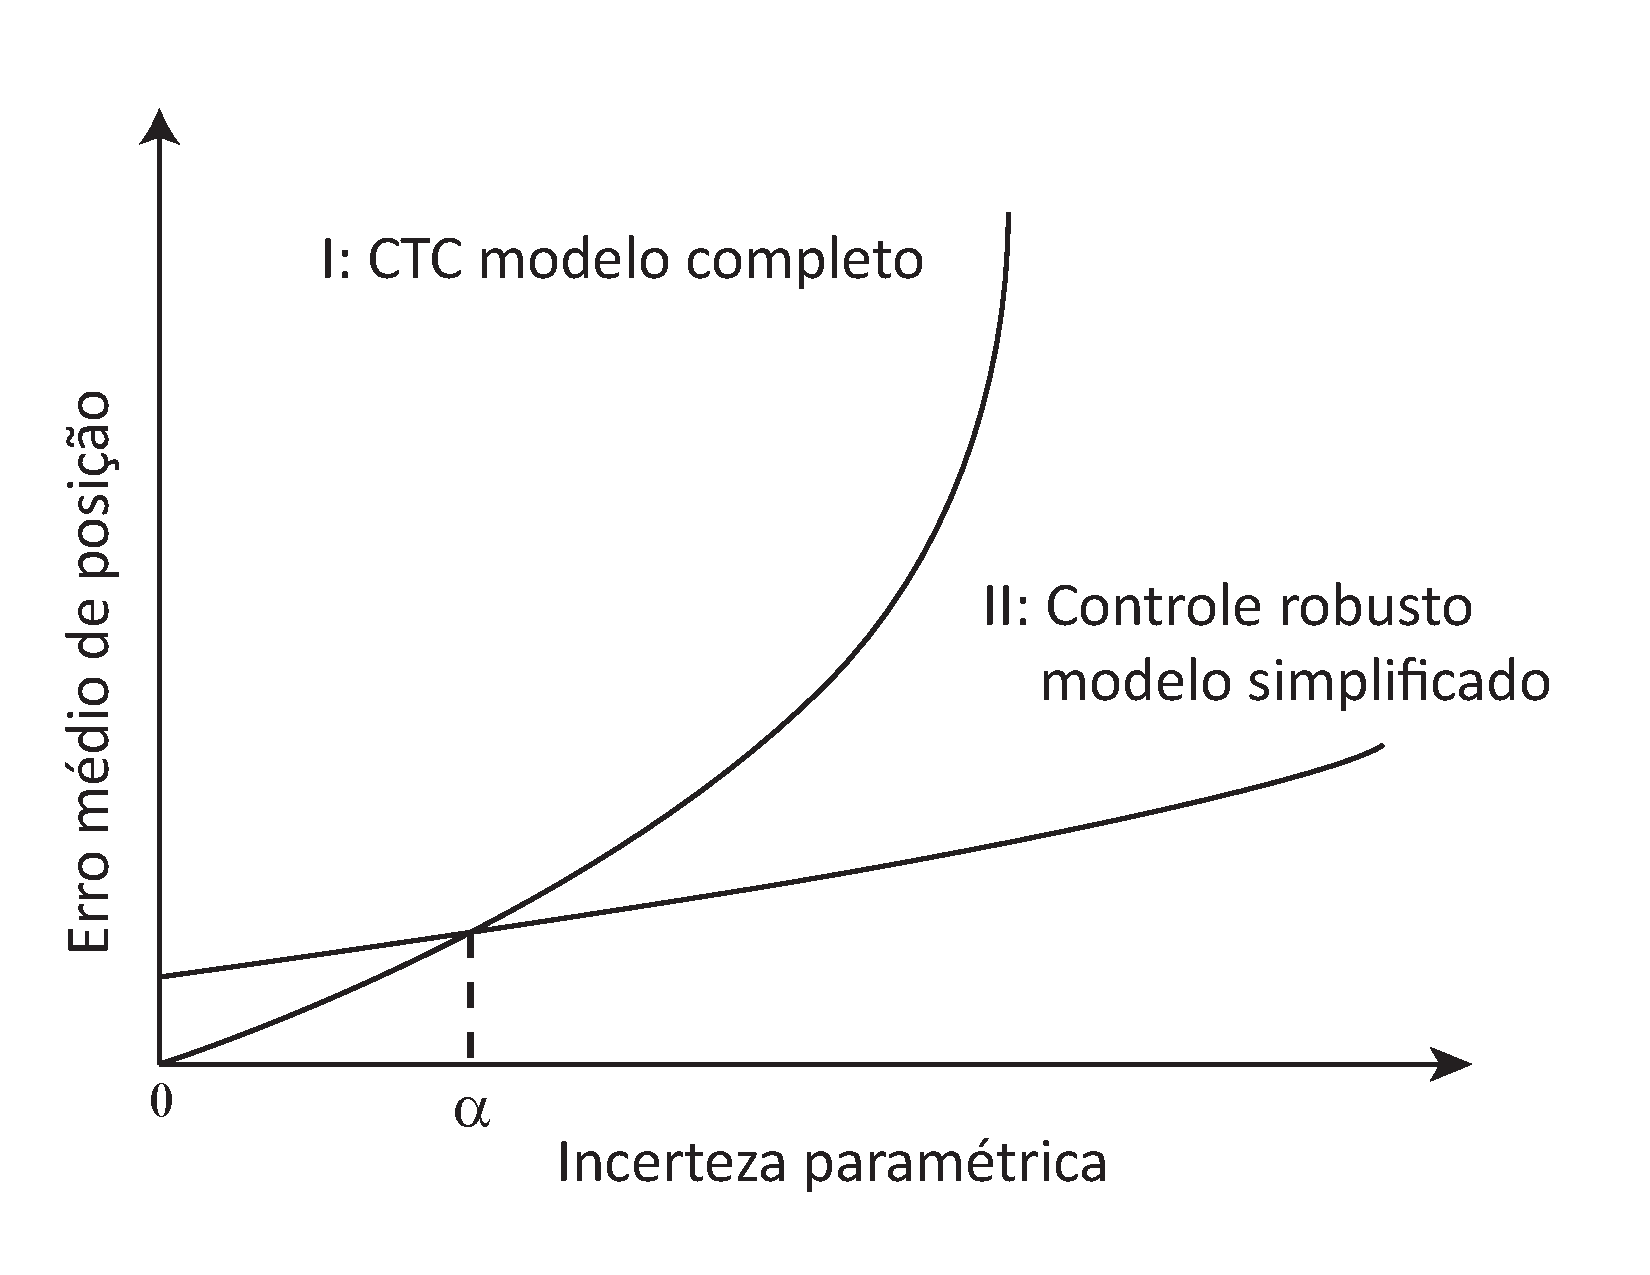
\includegraphics[scale=0.30]{Slotine.pdf} \\
        (Slotine 1985)
    \end{figure}  
\end{frame}

%\begin{frame}{Motiva\c{c}\~ao}
%    \framesubtitle{Controle}
%    \begin{block}{Controle robusto?}
%        Torna poss\'ivel garantir a converg\^encia do erro de controle para zero, mesmo com erros de modelagem \pause $\rightarrow$ compensa\c{c}\~ao din\^amica simplificada
%    \end{block}
%    \pause
%    \begin{exampleblock}{Exemplo}
%        Dado o seguinte sistema din\^amico:
%        $$ \mH(\mq) \ddot{\mq} + \mh (\mq, \dot{\mq}) = \mup $$
%        \'E poss\'ivel projetar uma lei de controle do tipo
%        $$ \mup = \underline{\mup}(t,\mq,\dot{\mq},\hat{\mh},\hat{\mH}) $$
%        que garante que $\me \rightarrow \mzr $ quando $t \rightarrow \infty$ \\
%        \vspace{6pt} \\
%        \pause $\therefore$  Lei de controle com menor custo computacional!
%    \end{exampleblock}
%\end{frame}

\begin{frame}{Objetivos}
	\begin{block}{}
		\pause
		\begin{itemize}
			\item[$\bullet$] Desenvolvimento de um algoritmo gerador de modelos din\^amicos completos de mecanismos paralelos, de forma impl\'icita \\[8pt]
			\pause
			\item[$\bullet$] Elabora\c{c}\~ao de uma metodologia de projeto de controlador n\~ao linear robusto, de alto desempenho, aplic\'avel a mecanismos paralelos \\[8pt]
			\pause
			\item[$\bullet$] Compara\c{c}\~ao da lei de controle proposta com outras leis de controle encontradas na literatura, atrav\'es de simula\c{c}\~oes e valida\c{c}\~oes experimentais \\[8pt]
	\end{itemize}
	\end{block}
\end{frame}

\begin{frame}{Escopo}
    \framesubtitle{Algoritmo de modelagem}
    \pause
    \begin{block}{Considera}
        \pause
        \begin{itemize}
            \item[--] In\'ercia distribu\'ida \\[6pt]
            \item[--] A\c{c}\~ao da gravidade \\[6pt]
            \item[--] <alert@4>Atritos nas juntas \\[6pt]
            \item[--] <alert@4>Din\^amica dos atuadores \\[6pt]
        \end{itemize}
    \end{block}
    \pause
    \pause
    \begin{block}{N\~ao considera}
        \pause
        \begin{itemize}
            \item[--] Folga nas juntas \\[6pt]
            \item[--] Deforma\c{c}\~oes \\[6pt]
        \end{itemize}
    \end{block}
\end{frame}

\begin{frame}{Escopo}
    \framesubtitle{Lei de controle proposta}
    \pause
    \begin{block}{Vari\'aveis controladas}
    	Posi\c{c}\~ao / orienta\c{c}\~ao do efetuador
    \end{block}
    \pause
    \begin{block}{Vari\'aveis monitoradas}
    	Coordenadas dos atuadores
    \end{block}
    \pause
    \begin{block}{Depend\^encia entre vari\'aveis controladas}
    	Controle centralizado baseado em modelo
    \end{block}
    \pause
   	\begin{block}{Estrat\'egia de controle}
    	Controle por modos deslizantes
    \end{block}
\end{frame}

\begin{frame}{Escopo}
    \framesubtitle{Lei de controle proposta}
    \begin{block}{Considera}
    	\begin{itemize}
    		\item[--] Incertezas param\'etricas \\[8pt]
    		\item[--] Erros na compensa\c{c}\~ao din\^amica \\[8pt]
    		\item[--] Din\^amica dos atuadores \\[8pt]
    	\end{itemize}
    \end{block}
    \pause
    \begin{block}{Objetivos}
    	\begin{itemize}
    		\item[--] Alta robustez \\[8pt]
    		\item[--] Alto desempenho em altas velocidades/acelera\c{c}\~oes \\[8pt]
    		\item[--] Baixo custo computacional \\[8pt]
    	\end{itemize}
    \end{block}
\end{frame}

\begin{frame}{Algoritmo de modelagem}
    \pause
    \begin{block}{Formula\c{c}\~ao impl\'icita}
        Torna poss\'ivel a implementa\c{c}\~ao em linguagens de programa\c{c}\~ao de alta efici\^encia computacional, como C++
    \end{block}
\end{frame}

\begin{frame}{Algoritmo de modelagem}
    \begin{block}{Met\'odos de modelagem din\^amica}
        \pause
        \begin{itemize}
            \item[--] Newton-Euler (1760)  \\[4pt]
            \item[--] <alert@3> Princ\'ipio de D'Alembert (1742) \\[4pt]
            \item[--] <alert@4> Lagrange (1788) \\[4pt]
            \item[--] <alert@4> Hamilton (1833) \\[4pt]
            \item[--] <alert@4> Gibbs-Appel (1879-1900) \\[4pt]
            \item[--] <alert@4> Maggi (1896) \\[4pt]
            \item[--] <alert@4> Boltzmann-Hamel (1901) \\[4pt]
            \item[--] Kane (1965) \\[4pt]
            \item[--] Udwadia-Kalaba (1992) \\[4pt]
            \item[--] Orsino (2015) \\[4pt]
        \end{itemize}
    \end{block}
\end{frame}

\begin{frame}{Algoritmo de modelagem}
    \begin{block}{Met\'odos que permitem formula\c{c}\~ao impl\'icita}
        \pause
        \begin{itemize}
            \item[--] Newton-Euler \\[4pt]
            \item[--] Kane \\[4pt]
            \item[--] Udwadia-Kalaba \\[4pt]
            \item[--] Orsino \\[4pt]
        \end{itemize}
    \end{block}
    \pause
    \begin{block}{M\'etodo escolhido}
        \pause
        M\'etodo Orsino: \pause Permite realizar a modelagem de maneira modular
    \end{block}
\end{frame}

\begin{frame}{Algoritmo de modelagem}
    \begin{figure}[!h]
        \centering
        \includegraphics[scale=0.45]{Modelagem.pdf} \\
        (Orsino 2016)
    \end{figure}  
\end{frame}

\begin{frame}{Algoritmo de modelagem}
    \framesubtitle{Seriais}
    \pause
    \begin{block}{Dados de entrada}
    	\begin{itemize}
    		\item[--] Par\^ametros de Denavit-Hartemberg ($a_i$, $\alpha_i$, $\theta_i$, $d_i$) \\[8pt]
    		\item[--] Posi\c{c}\~ao dos centros de massa em rela\c{c}\~ao aos sistemas $\ttB_i$ ($x_i$, $y_i$, $z_i$) \\[8pt]
    		\item[--] Massa $m_i$ de cada ligamento \\[8pt]
    		\item[--] Tensor de in\'ercia $\vct{\vI_i}_{\ttB_i \rl \ttB_i}$ em rela\c{c}\~ao ao centro de massa de cada ligamento \\[8pt]
    		\item[--] Vetor acelera\c{c}\~ao gravitacional escrito no sistema fixo (\vct{\vg}_{\ttN}) \\[8pt]
    	\end{itemize}
    \end{block}
\end{frame}

\begin{frame}{Algoritmo de modelagem}
    \framesubtitle{Seriais: Exemplo}
    \pause
    \begin{figure}[!h]
        \centering
        \includegraphics[scale=0.18]{RR.pdf}
    \end{figure}
\end{frame}

\begin{frame}{Algoritmo de modelagem}
    \framesubtitle{Seriais: Exemplo}
    \begin{table}[H]
		\begin{center}
		\begin{tabular}{|c|c|c|c|c|c|c|c|c|c|} 
			\hline
			\rule[-2mm]{0mm}{6mm}
			Ligamento & $a_i$ & $\alpha_i$ & $d_i$ & $\theta_i$ & x_i & y_i & z_i & m_i \\
			\hline
			\rule[-2mm]{0mm}{6mm}
			(1) & $l_1$ & $0$ & $0$ & $q_1(t)$ & $l_{g1} - l_1$ & 0 & 0 & m_1 \\
			\rule[-1mm]{0mm}{5mm}
			(2) & $l_2$ & $0$ & $0$ & $q_2(t)$ & $l_{g2} - l_2$ & 0 & 0 & m_2 \\
			\hline
		\end{tabular}
		\end{center}
	\end{table}
	$$ \vct{\vI_1}_{\ttB_1 \rl \ttB_1} = \begin{bmatrix} 0 & 0 & 0 \\ 0 & Jz_1 & 0 \\ 0 & 0 & Jz_1 \end{bmatrix} $$
	$$ \vct{\vI_2}_{\ttB_2 \rl \ttB_2} = \begin{bmatrix} 0 & 0 & 0 \\ 0 & Jz_2 & 0 \\ 0 & 0 & Jz_2 \end{bmatrix} $$
	$$ \vct{\vg}_{\ttN} = \begin{bmatrix} 0 & -g & 0 \end{bmatrix}^\msT $$
\end{frame}

\begin{frame}{Algoritmo de modelagem}
    \framesubtitle{Paralelos}
    \pause
    \begin{block}{Dados de entrada}
    	\begin{itemize}
    		\item[--] Modelo da plataforma/efetuador \\[8pt]
    		\item[--] Modelo das cadeias seriais \\[8pt]
    		\item[--] Matrizes constantes que descrevem a arquitetura do mecanismo ($\md$, $\mD$, $\mE$, $\mF$, $\mP$, $\mQ$, $\mR$) \\[8pt]
    	\end{itemize}
    \end{block}
\end{frame}

\begin{frame}{Algoritmo de modelagem}
    \framesubtitle{Paralelos: Exemplo}
    \pause
    \begin{figure}[!h]
        \centering
        \includegraphics[scale=0.4]{5Rscanf.pdf}
    \end{figure}
\end{frame}

\begin{frame}{Algoritmo de modelagem}
    \framesubtitle{Paralelos: Exemplo}
	$$ \mq\ssh = 
\begin{bmatrix}
1 & 0 & 0 \\
0 & 1 & 0 \\
\end{bmatrix}
\cdot
\mx_1(\mq_1)
+
\begin{bmatrix}
l_0 \\
0 \\
\end{bmatrix} $$
$$ \mq\ssh = 
\begin{bmatrix}
-1 & 0 & 0 \\
0 & 1 & 0 \\
\end{bmatrix}
\cdot
\mx_2(\mq_2)
+
\begin{bmatrix}
-l_0 \\
0 \\
\end{bmatrix} $$
\pause
$$ \overline{\mq}(\mq) =
\begin{bmatrix}
1 & 0 \\
0 & 1 \\
1 & 0 \\
0 & 1 \\
\end{bmatrix}
\cdot
\mq\ssh
-
\begin{bmatrix}
1 & 0 & 0 & 0 & 0 & 0 \\
0 & 1 & 0 & 0 & 0 & 0 \\
0 & 0 & 0 & -1 & 0 & 0 \\
0 & 0 & 0 & 0 & 1 & 0 \\
\end{bmatrix}
\cdot
\mx(\mq\cir)
-
\begin{bmatrix}
l_0 \\
0 \\
-l_0 \\
0 \\
\end{bmatrix}
= \mzr $$
\pause
$$ \overline{\momega}(\mq, \dot{\mq}) = \vct{\varnothing} $$    
\end{frame}

\begin{frame}{Algoritmo de modelagem}
    \framesubtitle{Paralelos: Exemplo}
    $$ \md = 
		\begin{bmatrix}
			l_0 &
			0 &
			-l_0 &
			0
		\end{bmatrix}^\msT $$
    %\begin{multicols}{2}
		$$ \mD = 
		\begin{bmatrix}
			1 & 0 \\
			0 & 1 \\
			1 & 0 \\
			0 & 1 \\
		\end{bmatrix} $$
		$$ \mE = 
		\begin{bmatrix}
			1 & 0 & 0 & 0 & 0 & 0 \\
			0 & 1 & 0 & 0 & 0 & 0 \\
			0 & 0 & 0 & -1 & 0 & 0 \\
			0 & 0 & 0 & 0 & 1 & 0 \\
		\end{bmatrix} $$
	%\end{multicols}
	$$ \mF = \mzr $$
	$$ 	\mP = \mQ = \mR = \vct{\varnothing} $$
\end{frame}

\begin{frame}{Controle}
    \framesubtitle{Lei de controle proposta}
    \pause
    \begin{block}{Modelo din\^amico}
    	$$ \mH(\mq)  \ddot{\mq}\ssh + \mh(\mq,\dot{\mq}\ssh) = \mup $$
    	Sendo:
    	$$ \mh(\mq,\dot{\mq}\ssh) = \mgamma(\mq) + \sum_{i=1}^{\nu\ssh} \sum_{j=1}^i \mgamma_{i,j}(\mq) \dot{q}\ssh_i \dot{q}\ssh_j $$
    \end{block}
    \pause
   	\begin{block}{Modelo din\^amico estimado}
    	$$ \hat{\mH}(\mq)  \ddot{\mq}\ssh + \hat{\mh}(\mq,\dot{\mq}\ssh) = \mup $$
    	Sendo:
    	$$ \hat{\mh}(\mq,\dot{\mq}\ssh) = \hat{\mgamma}(\mq) + \sum_{i=1}^{\nu\ssh} \sum_{j=1}^i \hat{\mgamma}_{i,j}(\mq) \dot{q}\ssh_i \dot{q}\ssh_j $$
   	\end{block}
\end{frame}

\begin{frame}{Controle}
    \framesubtitle{Lei de controle proposta}
   	\begin{block}{Medidores do erro de modelagem}
   		$$ \mDelta(\mq) = \mH(\mq)^\msI \hat{\mH}(\mq) - \mone $$
    	$$ \mdelta_0(\mq) = \mH(\mq)^\msI (\hat{\mgamma}(\mq) - \mgamma(\mq)) $$
    	$$ \mdelta_{i,j}(\mq) = \mH(\mq)^\msI (\hat{\mgamma}_{i,j}(\mq) - \mgamma_{i,j}(\mq)) $$
   	\end{block}
\end{frame}

\begin{frame}{Controle}
    \framesubtitle{Lei de controle proposta}
	\begin{block}{Lei de controle}
    	$$ \mup = \hat{\mh} + \hat{\mH}( \ddot{\mq}\ssh_d + \underline{\lambda}\dot{\me} + \underline{k} \sign(\dot{\me} + \underline{\lambda}\me) ) $$
    	\pause
    	Sendo:
    	$$ \diag(\underline{k})  = \meta + \mGamma |\ddot{\mq}\ssh_d + \underline{\lambda}\dot{\me}| + \sum_{i=1}^{\nu\ssh}\sum_{j=1}^{i} \meta_{i,j} |\dot{q}\ssh_i||\dot{q}\ssh_j| $$
    	$$ \mGamma = (\mone - |\mDelta|_{max} )^\msI |\mDelta|_{max} $$
    	$$ \meta = (\mone - |\mDelta|_{max} )^\msI ( | \mdelta_0 |_{max} + \diag(\eta \mone) ) $$
    	$$ \meta_{i,j} = (\mone - |\mDelta|_{max} )^\msI | \mdelta_{i,j} |_{max} $$
   	\end{block}
\end{frame}

\begin{frame}{Controle}
    \framesubtitle{Metodologia de projeto}
    \begin{block}{}
    	\begin{itemize}
    		\pause
			\item[$\bullet$] Discretizar o espa\c{c}o de trabalho em um n\'umero finito de pontos \\[8pt]
			\pause
			\item[$\bullet$] Para cada ponto, calcular $|\mDelta|$, $|\mdelta_0|$ e $|\mdelta_{i,j}|$ para todas as combina\c{c}\~oes poss\'iveis de par\^ametros, com os par\^ametros podendo assumir seu valor m\'inimo e seu valor m\'aximo \\[8pt]
			\pause
			\item[$\bullet$] Obter o valor m\'aximo de $|\mDelta|$, $|\mdelta_0|$ e $|\mdelta_{i,j}|$ para cada ponto. \\[8pt]
			\pause
			\item[$\bullet$] Obter o valor m\'aximo de $|\mDelta|$, $|\mdelta_0|$ e $|\mdelta_{i,j}|$ para o espa\c{c}o de trabalho, a partir do valor m\'aximo em cada ponto. \\[8pt]
		\end{itemize}
	\end{block}
\end{frame}

\begin{frame}{Controle}
    \framesubtitle{Vantagens da lei proposta}
    \begin{block}{}
    	\begin{itemize}
    		\pause
			\item[$\bullet$] Alto desempenho, mesmo em altas velocidades/acelera\c{c}\~oes \\[8pt]
			\pause
			\item[$\bullet$] Insens\'ivel incertezas param\'etricas \\[8pt]
			\pause
			\item[$\bullet$] Baixo custo computacional, visto que \'e poss\'ivel tabelar $\hat{\mH}$, $\hat{\mgamma}$ e $\hat{\mgamma}_{i,j}$\\[8pt]
			\pause
			\item[$\bullet$] Alta robustez \\[8pt]
		\end{itemize}
    \end{block}
\end{frame}

\begin{frame}{Resultados}
	\framesubtitle{Simula\c{c}\~oes}
	\pause
	\begin{block}{Mecanismo}
		2\underline{R}SU + \underline{P}PaP
	\end{block}
	\begin{figure}[!h]
        \centering
        \includegraphics[scale=0.25]{asym.png} \\
        (Orsino 2012)
    \end{figure}
\end{frame}

%\begin{frame}{Resultados}
%	\framesubtitle{Simula\c{c}\~oes}
%	\begin{block}{Par\^ametros do mecanismo}
%		\begin{multicols}{2}
%			\begin{itemize}
%				\item[-] $l_1 = 0.12 m$
%				\item[-] $l_2 = 0.15 m$
%				\item[-] $l_{g1} = 0.051 m$
%				\item[-] $l_{g2} = 0.086 m$
%				\item[-] $m_0 = 0 \, kg$
%				\item[-] $m_1 = 0.1645 kg$
%				\item[-] $m_2 = 0.1967 kg$
%				\item[-] $Jz_1 = 197.3 \cdot 10^{-6} kg\cdot m^2$
%				\item[-] $Jz_2 = 368.7 \cdot 10^{-6} kg\cdot m^2$
%				\item[-] $g = 9.8 m/s^2$
%			\end{itemize}
%		\end{multicols}
%	\end{block}
%	\begin{block}{Par\^ametros estimados}
%		\begin{multicols}{2}
%			\begin{itemize}
%				\item[-] $\hat{l}_1 = 0.12 m$
%				\item[-] $\hat{l}_2 = 0.15 m$
%				\item[-] $\hat{l}_{g1} = 0.06 m$
%				\item[-] $\hat{l}_{g2} = 0.075 m$
%				\item[-] $\hat{m}_0 = 0 \, kg$
%				\item[-] $\hat{m}_1 = 0.143 kg$
%				\item[-] $\hat{m}_2 = 0.171 kg$
%				\item[-] $\hat{J}z_1 = 171.6 \cdot 10^{-6} kg\cdot m^2$
%				\item[-] $\hat{J}z_2 = 320.6 \cdot 10^{-6} kg\cdot m^2$
%				\item[-] $\hat{g} = 9.8 m/s^2$
%			\end{itemize}
%		\end{multicols}
%	\end{block}
%\end{frame}

\begin{frame}{Resultados}
	\framesubtitle{Simula\c{c}\~oes}
	\begin{block}{Trajet\'oria de refer\^encia}
		%$$
		%\begin{cases}
		%	q\ssh_{1 \, d}(t) = 0.07 \cos(28.57 t) \\
		%	q\ssh_{2 \, d}(t) = 0.17 + 0.07 \sin(28.57 t) \\
		%\end{cases}
		%$$
		C\'irculo com $740mm$ de di\^ametro, velocidade tangencial de $1.0m/s$.
	\end{block}
	\begin{figure}[!h]
        \centering
        \includegraphics[scale=0.17]{Workspace2.jpg}
    \end{figure}
\end{frame}

\begin{frame}{Resultados}
	\framesubtitle{Simula\c{c}\~oes}
	%%\begin{block}{Condi\c{c}\~oes iniciais}
	%%	$$
	%%	\begin{cases}
	%%		q\ssh_1(0) = 0.07 m\\
	%%		q\ssh_2(0) = 0.17 m \\
	%%		\dot{q}\ssh_1(0) = 0 \\
	%%		\dot{q}\ssh_2(0) = 0 \\
	%%	\end{cases}
	%%	$$
	%%\end{block}
	\begin{block}{Par\^ametros do controlador}
		\begin{itemize}
			\item[--] $ \lambda = 50.0 \Rightarrow$ Tempo de assentamento de $0.08s$ \\[8pt]
			\item[--] $ \eta = 20.0 \Rightarrow$ Tempo de chegada a $\ms=\mzr$ menor que $0.05s$ \\[8pt]
		\end{itemize}
	\end{block}
	\begin{block}{Fun\c{c}\~ao de satura\c{c}\~ao}
		$$f_{sat}(x) = \tanh(20x)$$
	\end{block}
	\begin{figure}[!h]
        \centering
        \includegraphics[scale=0.20]{Tanh2.pdf}
    \end{figure}
\end{frame}

\begin{frame}{Resultados}
	\framesubtitle{Simula\c{c}\~oes}
	
\end{frame}

\begin{frame}{Resultados}
	\framesubtitle{Simula\c{c}\~oes}
	\begin{figure}[!h]
        \centering
        \includegraphics[scale=0.45]{Torque1.pdf}
    \end{figure}
\end{frame}

\begin{frame}{Resultados}
	\framesubtitle{Simula\c{c}\~oes}
	\begin{figure}[!h]
        \centering
        \includegraphics[scale=0.45]{Torque2.pdf}
    \end{figure}
\end{frame}

\begin{frame}{Resultados}
	\framesubtitle{Simula\c{c}\~oes}
	\begin{figure}[!h]
        \centering
        \includegraphics[scale=0.45]{Forca3.pdf}
    \end{figure}
\end{frame}

\begin{frame}{Resultados}
	\framesubtitle{Simula\c{c}\~oes}
	\begin{figure}[!h]
        \centering
        \includegraphics[scale=0.45]{ex.pdf}
    \end{figure}
\end{frame}

\begin{frame}{Resultados}
	\framesubtitle{Simula\c{c}\~oes}
	\begin{figure}[!h]
        \centering
        \includegraphics[scale=0.45]{ey.pdf}
    \end{figure}
\end{frame}

\begin{frame}{Resultados}
	\framesubtitle{Simula\c{c}\~oes}
	\begin{figure}[!h]
        \centering
        \includegraphics[scale=0.45]{ez.pdf}
    \end{figure}
\end{frame}

\begin{frame}{Resultados}
	\framesubtitle{Simula\c{c}\~oes}
	\begin{figure}[!h]
        \centering
        \includegraphics[scale=0.45]{sx.pdf}
    \end{figure}
\end{frame}

\begin{frame}{Resultados}
	\framesubtitle{Simula\c{c}\~oes}
	\begin{figure}[!h]
        \centering
        \includegraphics[scale=0.45]{sy.pdf}
    \end{figure}
\end{frame}

\begin{frame}{Resultados}
	\framesubtitle{Simula\c{c}\~oes}
	\begin{figure}[!h]
        \centering
        \includegraphics[scale=0.45]{sz.pdf}
    \end{figure}
\end{frame}

\begin{frame}{Conclus\~oes parciais}
	\begin{block}{}
		\begin{itemize}
			\pause
			\item[$\bullet$] \'E fundamental a utiliza\c{c}\~ao linguagens de alta efici\^encia computacional para realizar  simula\c{c}\~oes din\^amicas de modelos completos de mecanismos complexos
			\pause
			\item[$\bullet$] \'E poss\'ivel obter alto desempenho no controle mecanismos paralelos em altas velocidades/acelera\c{c}\~oes utilizando t\'ecnicas de controle n\~ao linear robusto, mesmo com altos n\'iveis de incertezas param\'etricas
		\end{itemize}
	\end{block}
\end{frame}

\begin{frame}{Publica\c{c}\~oes}
    \begin{block}{BioRob 2014}
        ``Development of a Controller of a 3-Dof Robotic Platform for User Interaction in Rehabilitation Therapies''
    \end{block}
    \begin{figure}[!h]
        \centering
        \includegraphics[scale=0.45]{TF.jpg}
    \end{figure}
\end{frame}

\begin{frame}{Publica\c{c}\~oes}
    \begin{block}{Cap\'itulo de livro}
        ``Dynamic Modelling and Control of balanced parallel mechanisms''
    \end{block}
    \begin{figure}[!h]
        \centering
        \includegraphics[scale=0.50]{5R.pdf}
    \end{figure}
\end{frame}

\begin{frame}{Publica\c{c}\~oes}
    \begin{block}{International Journal of Mechanisms and Robotic Systems}
        ``A new approach for obtaining the dynamic balancing conditions in serial mechanisms''
    \end{block}
    \begin{figure}[!h]
        \centering
        \includegraphics[scale=0.30]{RRRESPACIALW.pdf}
    \end{figure}
\end{frame}

%\begin{frame}{T\'opicos futuros}
%\end{frame}

\begin{frame}{Cronograma}
    \begin{itemize}
    	\pause
		\item[(1)]<2-| alert@2> Inclus\~ao de atritos nas juntas e da din\^amica eletro-mec\^anica dos atuadores no algoritmo de modelagem \\[4pt]
		\item[(2)]<3-| alert@3> Projeto e simula\c{c}\~ao de controlador por tens\~ao para os mecanismos 5R e 2\underline{R}SU+\underline{P}PaP \\[4pt]
		\item[(3)]<4-| alert@4> Valida\c{c}\~ao experimental dos controladores projetados, utilizando os prot\'otipos \\[4pt]
		\item[(4)]<5-| alert@5> Escrever artigos sobre modelagem e controle de mecanismos paralelos \\[4pt]
		\item[(5)]<6-| alert@6> Avalia\c{c}\~ao geral dos resultados \\[4pt]
		\item[(6)]<7-| alert@7> Preparo da tese \\[4pt]
    \end{itemize}
\end{frame}

\begin{frame}{Cronograma}
    \begin{table}[H]
		\begin{center}
			%\caption[Cronograma]{Cronograma -- Planejamento de Atividades por quadrimestre}
			\begin{tabular}{|c|c|c|c|c|c|} 
				\hline
				\rule[-2mm]{0mm}{6mm}
				Ativ./Quad. & $3^o/16$ & $1^o/17$ & $2^o/17$ & $3^o/17$ \\
				\hline
				\rule[-2mm]{0mm}{6mm}
				(1) & \rule[0mm]{10mm}{2mm} &   &  &    \\
				\rule[-1mm]{0mm}{5mm}
				(2) & \rule[0mm]{10mm}{2mm} & \rule[0mm]{10mm}{2mm} &  &    \\
				\rule[-1mm]{0mm}{5mm}
				(3) &  & \rule[0mm]{10mm}{2mm} & \rule[0mm]{10mm}{2mm} &     \\
				\rule[-1mm]{0mm}{5mm}
				(4) &   & \rule[0mm]{10mm}{2mm} & \rule[0mm]{10mm}{2mm} & \rule[0mm]{10mm}{2mm}    \\
				\rule[-1mm]{0mm}{5mm}
				(5) &   &  &  &  \rule[0mm]{10mm}{2mm}   \\
				\rule[-1mm]{0mm}{5mm}
				(6) &   & \rule[0mm]{10mm}{2mm} & \rule[0mm]{10mm}{2mm}  &  \rule[0mm]{10mm}{2mm}  \\
				\hline
			\end{tabular}
			%\label{crono}
		\end{center}
	\end{table}
\end{frame}

%-----------------------------------------------------------------------------------------------------------------------------------

\end{document}